\documentclass{article}

\usepackage{circuitikz} %Für die Schaltpläne
\usepackage[T1]{fontenc} 
\usepackage[utf8]{inputenc}
\usepackage{amsmath}
\usepackage{amssymb}
\usepackage{fancyhdr}
\usepackage{graphicx}
\usepackage{hyperref}
\usepackage{subcaption}
\usepackage{tikz}
\usepackage{../assets/scripts/tex/color-env}
\usepackage[ngerman]{babel}



    \usetikzlibrary{arrows}
    \usetikzlibrary{arrows.meta,topaths}
    \usetikzlibrary{bending}
    \usetikzlibrary{calc}
\title{Elektrotechnik 1 Praktikum 1}


\usepackage[
  includehead,
  headheight = 17mm,
  footskip = \dimexpr\headsep+\ht\strutbox\relax,
  tmargin = 0mm,
  bmargin = \dimexpr17mm+2\ht\strutbox\relax,
]{geometry}

\usepackage{anyfontsize}

\usepackage{xcolor}

\definecolor{DarkGreenBlue}{HTML}{264653}
\definecolor{LightGreenBlue}{HTML}{2A9D8F}
\definecolor{LightOrange}{HTML}{E9C46A}
\definecolor{DarkOrange}{HTML}{F4A261}
\definecolor{RedOrange}{HTML}{E76F51}
\definecolor{BrightRed}{HTML}{D62828}
\definecolor{DeepBlue}{HTML}{003049}



\pagestyle{fancy}
\fancyhead[L]{\leftmark}
\fancyhead[R]{}
\fancyfoot[L]{}
\fancyfoot[C]{\thepage}
\fancyfoot[R]{
\includegraphics[scale=0.2]{../assets/images/haw.jpg}}
\renewcommand\headrulewidth{0.5pt}


\begin{document}



\begin{tikzpicture}[overlay,remember picture]
  \thispagestyle{empty}
  \fill[black!2] (current page.south west) rectangle (current page.north east);

  \begin{scope}[transform canvas ={rotate around ={45:($(current page.north west)+(-.5,-6)$)}}]

    \shade[rounded corners=18pt, left color=DarkGreenBlue, right color=LightGreenBlue] ($(current page.north west)+(-.5,-6)$) rectangle ++(9,1.5);

  \end{scope}

  \begin{scope}[transform canvas ={rotate around ={45:($(current page.north west)+(.5,-10)$)}}]

    \shade[rounded corners=18pt, left color=LightOrange,right color=DarkOrange] ($(current page.north west)+(0.5,-10)$) rectangle ++(15,1.5);

  \end{scope}

  \begin{scope}[transform canvas ={rotate around ={45:($(current page.north west)+(0.5,-10)$)}}]

    \shade[rounded corners=8pt, right color=DarkOrange, left color=LightOrange] ($(current page.north west)+(1.5,-9.55)$) rectangle ++(7,.6);

  \end{scope}

  \begin{scope}[transform canvas ={rotate around ={45:($(current page.north)+(-1.5,-3)$)}}]

    \shade[rounded corners=12pt, left color=DeepBlue!80, right color=DeepBlue!60] ($(current page.north)+(-1.5,-3)$) rectangle ++(9,0.8);

  \end{scope}

  \begin{scope}[transform canvas ={rotate around ={45:($(current page.north)+(-3,-8)$)}}]

    \shade[rounded corners=28pt, left color=BrightRed, right color=BrightRed!80] ($(current page.north)+(-3,-8)$) rectangle ++(15,1.8);

  \end{scope}

  \begin{scope}[transform canvas ={rotate around ={45:($(current page.north west)+(4,-15.5)$)}}]

    \shade[rounded corners=25pt, left color=RedOrange, right color=DarkOrange] ($(current page.north west)+(4,-15.5)$) rectangle ++(30,1.8);

  \end{scope}

  \begin{scope}[transform canvas ={rotate around ={45:($(current page.north west)+(13,-10)$)}},]

    \shade[rounded corners=22pt, left color=DeepBlue,right color=DarkGreenBlue] ($(current page.north west)+(13,-10)$) rectangle ++(15,1.5);

  \end{scope}

  \begin{scope}[transform canvas ={rotate around ={45:($(current page.north west)+(18,-8)$)}},]

    \shade[rounded corners=8pt, left color=DarkOrange] ($(current page.north west)+(18,-8)$) rectangle ++(15,0.6);

  \end{scope}

  \begin{scope}[transform canvas ={rotate around ={45:($(current page.north west)+(19,-5.65)$)}},]

    \shade[rounded corners=12pt, left color=RedOrange] ($(current page.north west)+(19,-5.65)$) rectangle ++(15,0.8);

  \end{scope}

  \begin{scope}[transform canvas ={rotate around ={45:($(current page.north west)+(20,-9)$)}}]

    \shade[rounded corners=20pt, left color=BrightRed, right color=BrightRed!80] ($(current page.north west)+(20,-9)$) rectangle ++(14,1.2);

  \end{scope}

  \draw[ultra thick,gray] ($(current page.center)+(5,2)$) -- ++(0,-3cm) node[midway,left=0.25cm,text width=5cm,align=right,black!75]{{\fontsize{25}{30} \selectfont \bf Elektronik 1\\[10pt] Praktikum 2}} node[midway,right=0.25cm,text width=6cm,align=left,orange]{{\fontsize{70}{86} \selectfont 2020}};

  \node at ($(current page.center)+(0,-4)$) {{\fontsize{60}{72} \selectfont Diode}};

  \node[text width=8cm,align=center] at ($(current page.center)+(0,-6.5)$) {{\fontsize{16}{20} \selectfont \textcolor{orange}{ \bf \today}} \\[3pt] Florian Tietjen\\[3pt] Eric Antosch};

\end{tikzpicture}
\newpage
\thispagestyle{empty}

\tableofcontents


\newpage


\section{Durchlasskennlinien von Germanium- und Siliziumdiode}
\begin{task}
  TIn der ersten Aufgabe wollen wir die Kennlinien einer AA138 Germaniumdiode
  und einer 1N4148 Siliziumdiode mithilfe des X-Y-Schreibers des Oszilloskops aufnehmen.
\end{task}

\begin{figure}[h]
  \begin{center}
    \begin{circuitikz}[european]
      \draw (0,0) to[vsource, l=$U_0$] (0,4) to[diode, l_=$D$] (4,4) to[R, l_=$R_v$] (4,0) to[short] (0,0);
      \draw (1,4) to[short] (1,5) to[voltmeter, l=$U_x$] (3,5) to[short] (3,4);
      \draw (4,3) to[short] (5,3) to[voltmeter, l=$U_y$] (5,1) to[short] (4,1);
    \end{circuitikz}
    \caption{Aufbauzeichnung der Messung mithilfe des X-Y-Schreibers}
  \end{center}
\end{figure}

\begin{devlist}
  T\begin{itemize}
    \item X-Y-Schreiber
    \item Gleichspannungsgenerator
    \item AA138 Germaniumdiode
    \item 1N4148 Siliziumdiode
  \end{itemize}
\end{devlist}

\newpage

\subsection{Vorbereitung}

\begin{figure}[h]
  \centering
  \begin{subfigure}[b]{0.4\textwidth}
    \centering
    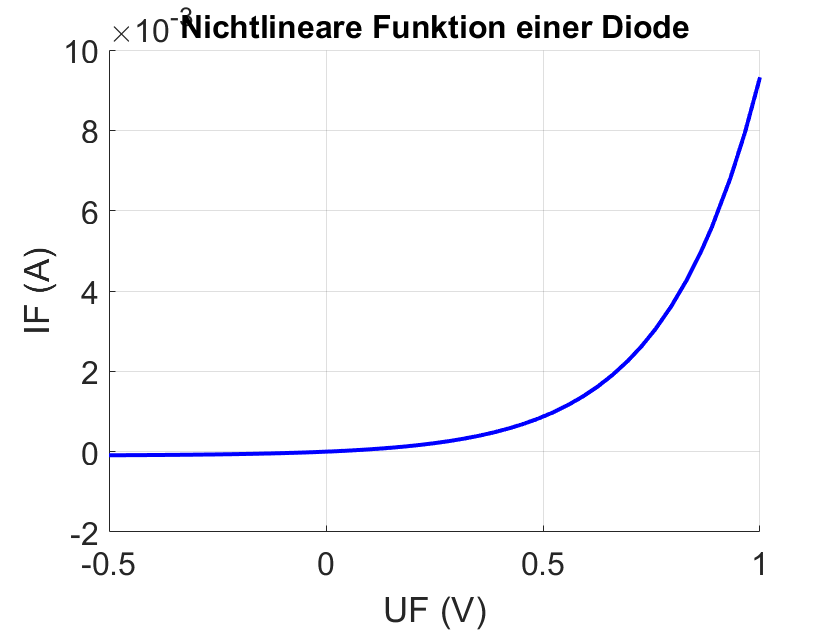
\includegraphics[width=\textwidth]{../assets/images/EL1P2/VorbereitungAA138.png}
    \caption{Kennlinie der AA138 Germaniumdiode}
  \end{subfigure}
  \hfill
  \begin{subfigure}[b]{0.4\textwidth}
    \centering
    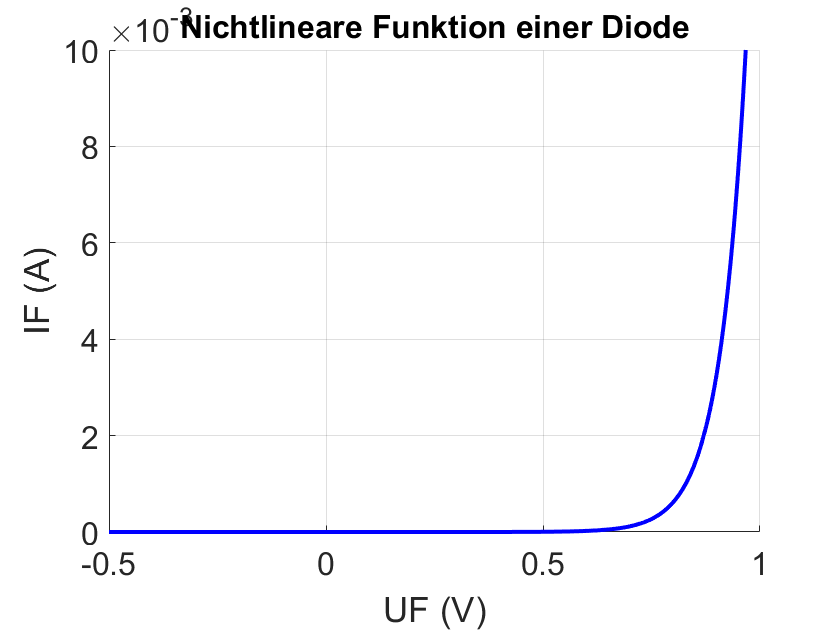
\includegraphics[width=\textwidth]{../assets/images/EL1P2/Vorbereitung1N4148.png}
    \caption{Kennlinie der 1N4148 Siliziumdiode}
  \end{subfigure}
  \caption{Die beiden Kennlinien der Dioden simuliert mit Shockley in Matlab}
\end{figure}

\subsection{Versuchsdurchführung}

Wir messen mithilfe des X-Y-Schreibers, wie im Versuchsaufbau gezeigt, den Strom über die Diode indirekt mithilfe der Spannung 
über den Vorwiderstand (Shunt). Die Spannung über die Diode messen wir einfach direkt mit den X-Eingängen des Schreibers. Den Strom durch den Schaltkreis regeln wir bis zu einem Stromfluss von 10mA hoch und nehmen dabei die 
Kennlinie der jeweiligen Diode auf.
\newpage
\subsection{Auswertung}

Wir legen an die Kennlinien jeweils eine Tangente an die Stelle $y=2mA$ und bestimmen daraus die Steigung und damit den differentiellen Widerstand der Diode:
\begin{figure}[h]
  \centering
  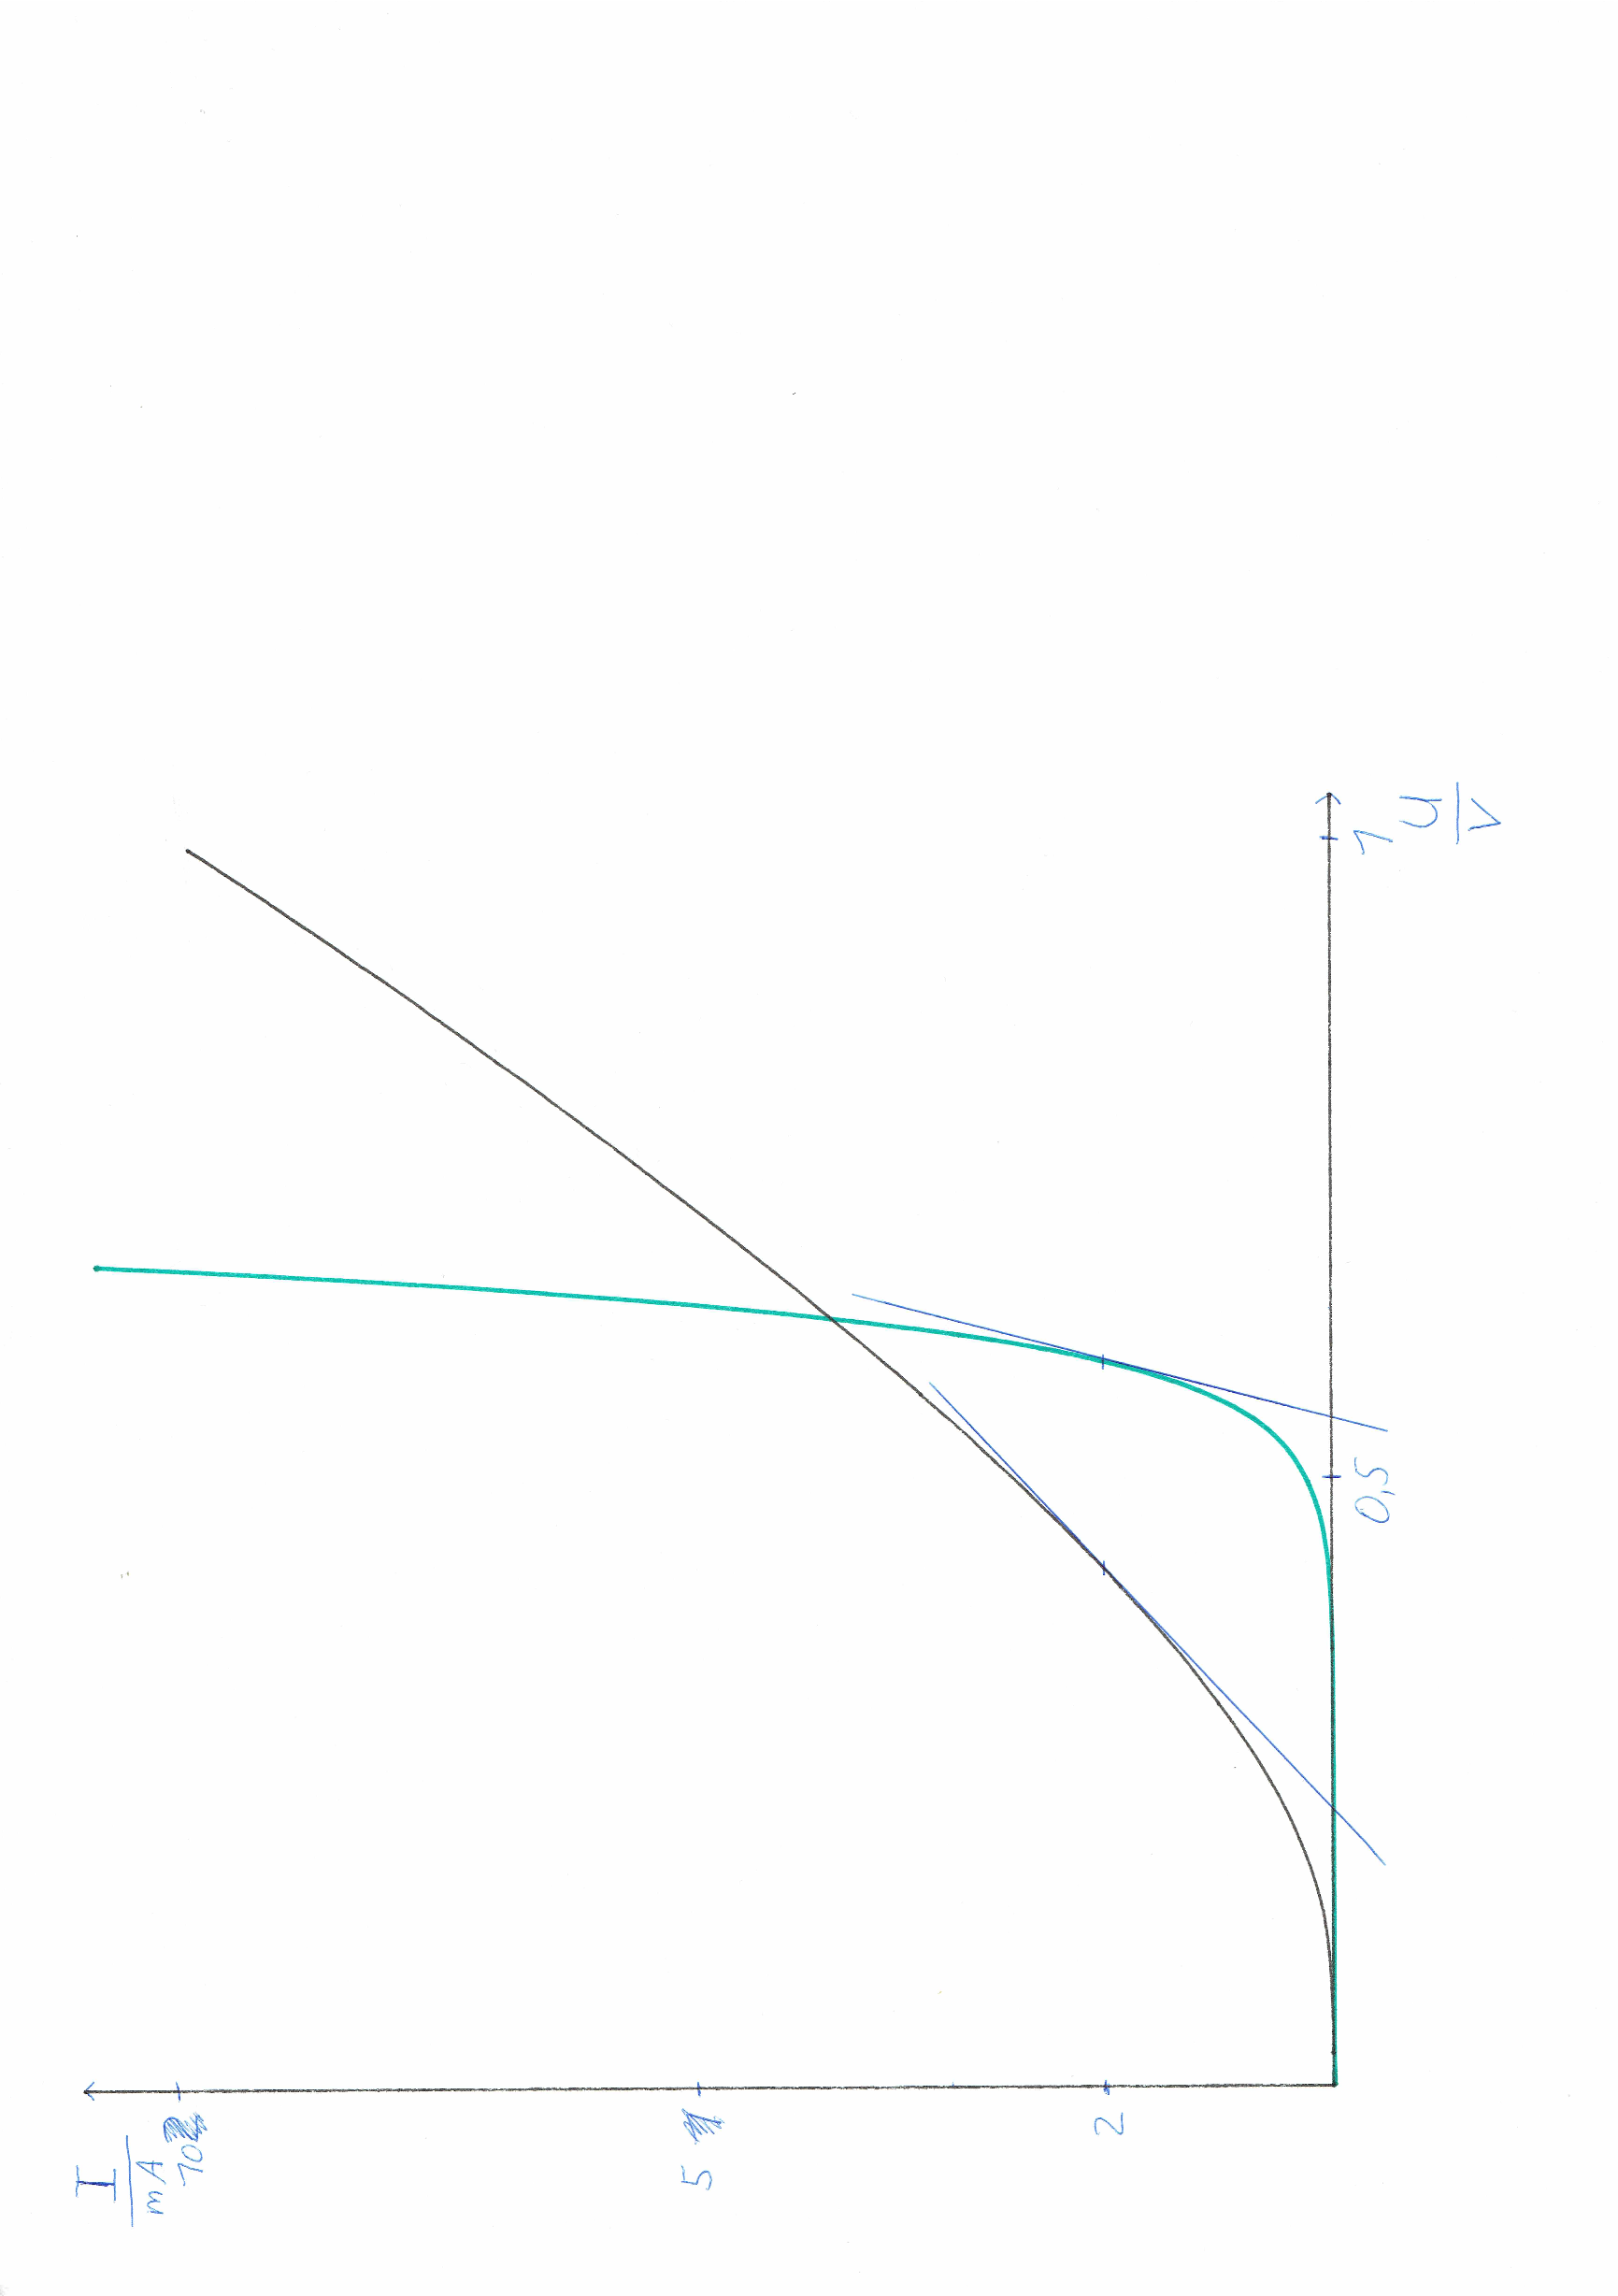
\includegraphics[scale=0.4, angle=-90]{../assets/images/EL1P2/ScanXY.PDF}
  \caption{Ergebnis des Aufnehmen der Kennlinie mit dem XY-Schreiber. (Blau 1N4148, Schwarz AA138)}
  \label{fig:xy}
\end{figure}

Wir erkennen, dass die Diodenkennlinie der Siliziumdiode um einiges stärker definiert ist und ihre Vorwärtspannung ab einem bestimmten Punkt einen stark expotentiellen Verlauf annimmt. Das ist auch mit ein Grund, warum Germaniumdioden heutzutage einen weitaus geringeren Stellenwert haben als Siliziumdioden, da sich Siliziumdioden besser vorhersagen und am Computer quantisieren lassen. Für die Siliziumdiode erhalten wir einen differentiellen Leitwert von $$G_{Si_{d}}= \frac{2mA-0,2mA}{0,6V-0,5V} = \frac{1,8mA}{0,1V} = 0,018S$$, also $$r_{Si_{d}} = \frac{1}{G_{Si_{d}}} = \frac{1}{0,018S} = 55,5\Omega.$$
Für die Germaniumdiode bekommen wir mit der Grafik nun einen differentiellen Leitwert von $$G_{Ge_{d}} = \frac{2mA-1,5mA}{0,4V-0,3V} = \frac{0,5mA}{0,1V} = 0,005S$$, also $$r_{Ge_{d}} = \frac{1}{G_{Ge_{d}}} = \frac{1}{0,005S} = 200\Omega.$$


\newpage

\section{Durchlasskennlinien der Siliziumdiode in halblogarithmischer Darstellung}
\begin{task}
  TIn diesem Versuch wollen wir erneut die Kennlinie der 1N4148 Siliziumdiode aufnehmen, wobei wir sowohl mehr Messpunkte als auch 
  eine halblogarithmische Darstellung wählen.
\end{task}

\begin{figure}[h]
  \begin{center}
    \begin{circuitikz}[european]
      \draw (0,0) to[vsource, l=$U_0$] (0,4) to[diode, l_=$D$] (4,4) to[R, l_=$R_v$] (4,0);
      \draw (0,0) to[ammeter] (4,0);
      \draw (1,4) to[short, *-] (1,5) to[voltmeter, l=$U_x$] (3,5) to[short, -*] (3,4);
    \end{circuitikz}
    \caption{Aufbauzeichnung der Messung mithilfe des MetraHit Tech Multimeter}
  \end{center}
\end{figure}

\begin{devlist}
  T\begin{itemize}
    \item Multimeter MetraHit X-TRA
    \item Gleichstromgenerator
    \item 1N4148 Siliziumdiode
  \end{itemize}
\end{devlist}
\newpage
\subsection{Vorbereitung}

\begin{figure}[h]
  \centering
  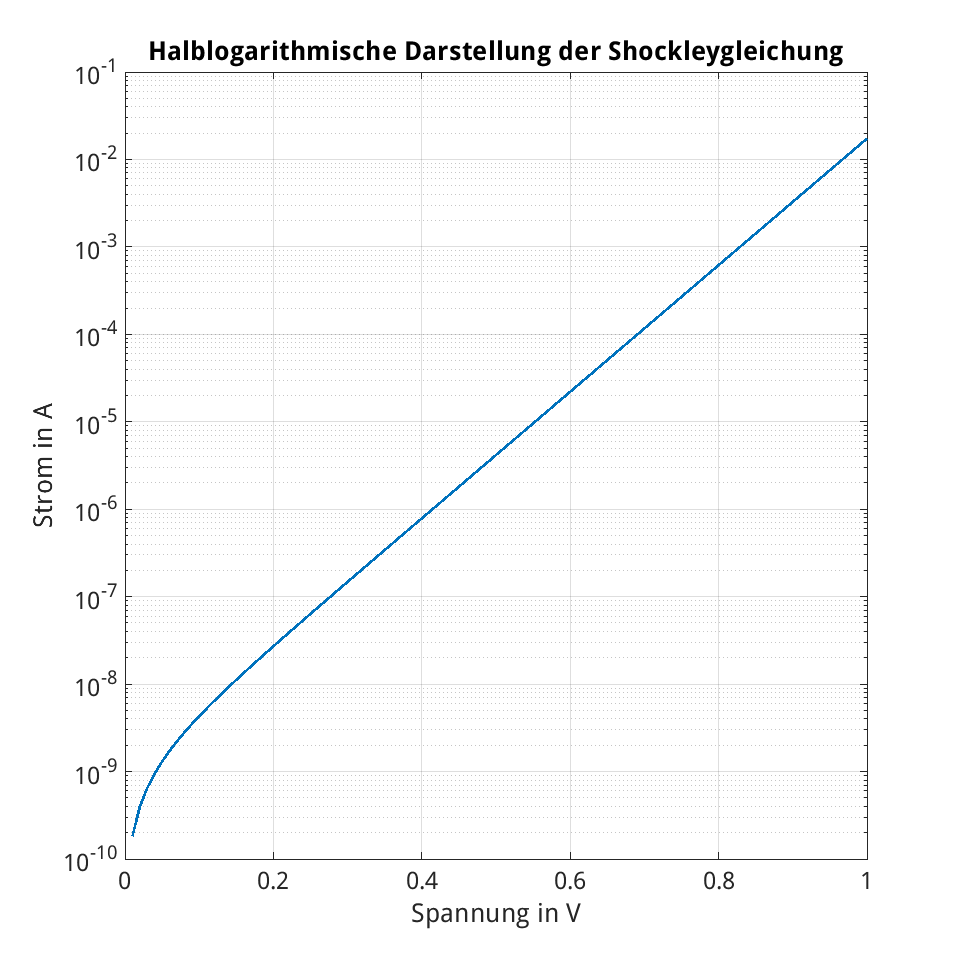
\includegraphics[scale=0.4]{../assets/images/EL1P2/VorbereitungSemilogDiode2.png}
  \caption{Semilogarithmische Darstellung der Shockleygleichung mit Matlab}
  \label{fig:vsemilog}
\end{figure}

Mithilfe von Matlab und der Shockleygleichung lässt sich eine halblogarithmische Darstellung der Diodenkennlinie erstellen, die man hier als stark linear erkennen kann.

\subsection{Versuchsdurchführung}

Wir lassen die Schaltung aus Aufgabe 1 weitesgehend aufgebaut und legen jetzt an die entsprechenden Stellen Multimeter(MetraHit Tech) an.

\begin{table}[h]
  \begin{center}
\begin{tabular}{|c|c|}
  \hline
  $I_{f}$ & $U_{f}$  \\
  \hline
  $10\mu A$ & 0,396V\\
  \hline
  $20\mu A$ & 0,433V\\
  \hline
  $50\mu A$ & 0,4761V\\
  \hline
  $100\mu A$ & 0,5079V\\
  \hline
  $200\mu A$ & 0,5418V\\
  \hline
  $500\mu A$ & 0,5873\\
  \hline
  $1mA$ & 0,6219V\\
  \hline
  $2mA$ & 0,6551V\\
  \hline
  $5mA$ & 0,7018V\\
  \hline
  $10mA$ & 0,7393V\\
  \hline
\end{tabular}
\caption{Messwerte, die mit dem Multimeter aufgenommen wurden in tabellarischer Form}
\end{center}
\end{table}

\begin{figure}[h]
  \begin{center}
    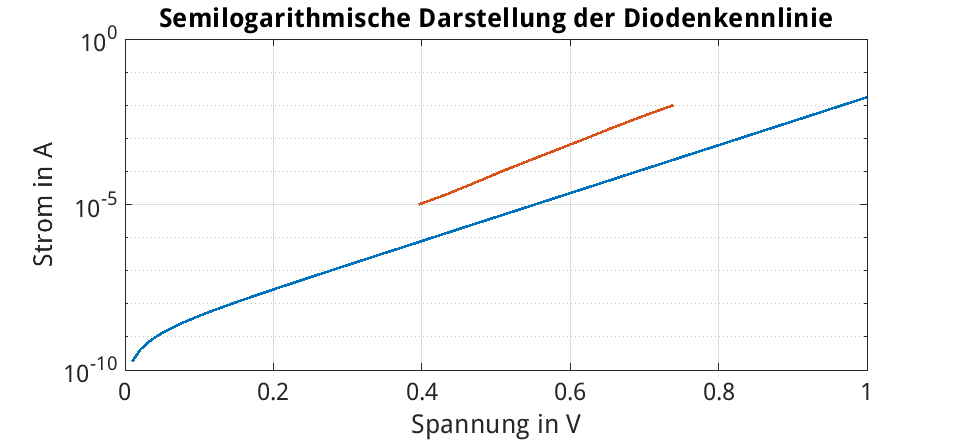
\includegraphics[scale=0.6]{../assets/images/EL1P2/SemilogDiodeVergleich.png}
    \caption{Semilogarithmische Darstellung der Diodenkennlinie mit Matlab}
  \end{center}
\end{figure}

Hier ist nun die Diodenkennlinie aus der Vorbereitung mit der neuen Kennlinie aus den Messwerten (orange) dargestellt.
\newpage
\subsection{Auswertung}

Es ist interessant, dass sowohl die Diodengleichung als auch die Messergebnisse zu sehr ähnlichen Grafiken führen, die nahezu linear sind. Dies ist jedoch nicht sehr verwunderlich, da in der Shockleygleichung auch ein Term mit $e$ vorkommt. Der Versatz, der sich zwischen beiden Kennlinie ergibt, kann aus vielen Faktoren entstanden seien, die aus der empfindlichen Art der Diode entstehen können. Dadurch, dass Halbleiterelemente zudem sehr temperaturabhängig sind, kann auch die Raumtemperatur des Labors eine Rollen spielen.

\newpage

\section{Einweggleichrichterschaltung}
\begin{task}
  TIn diesem Versuch wollen wir die Eigenschaften einer Einweggleichrichterschaltung mithilfe der uns 
  vermittelten Methoden analysieren und auswerten.
\end{task}

\begin{devlist}
  T\begin{itemize}
    \item Oszilloskop
    \item Funktionsgenerator
    \item Multimeter
    \item Lastwiderstand
    \item Kondensator
    \item 1N4148 Siliziumdiode
  \end{itemize}
\end{devlist}

\begin{figure}[h]
  \begin{center}
    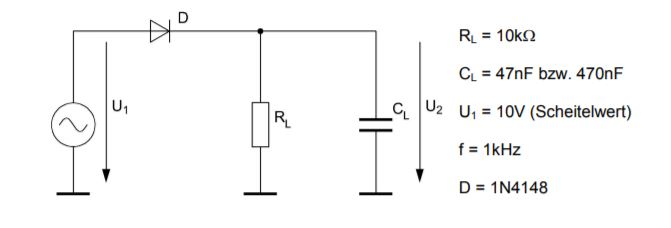
\includegraphics{../assets/images/EL1P2/aufgabe 3 schaltung.JPG}
    \caption{Einweggleichrichterschaltung mit Glättungskondensator}
  \end{center}
\end{figure}

\subsection{Darstellung der Zeitverläufe von $U_1$ und $U_2$}

\begin{figure}[h]
  \begin{center}
    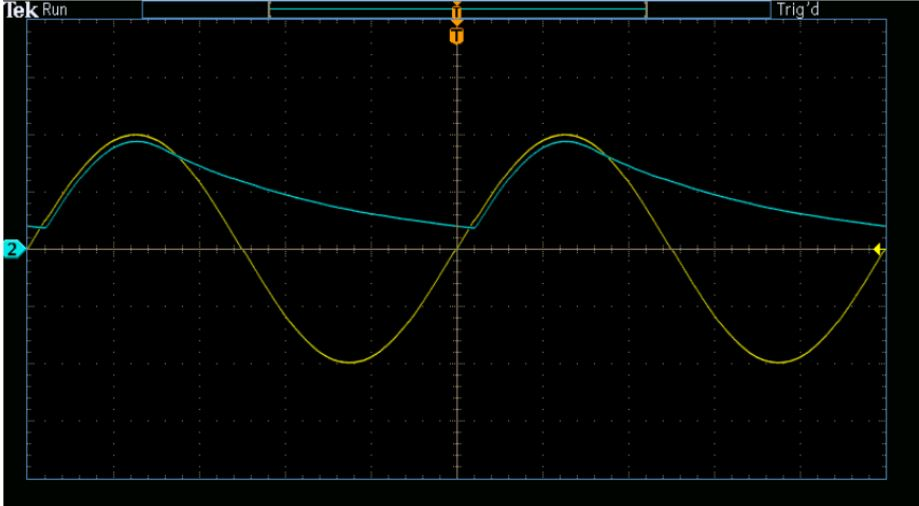
\includegraphics[scale=0.6]{../assets/images/EL1P2/aufgabe 3 47n.JPG}
    \caption{Spannungsverlauf bei $C_L$ = 47nF}
  \end{center}
\end{figure}

\begin{figure}[h]
  \begin{center}
    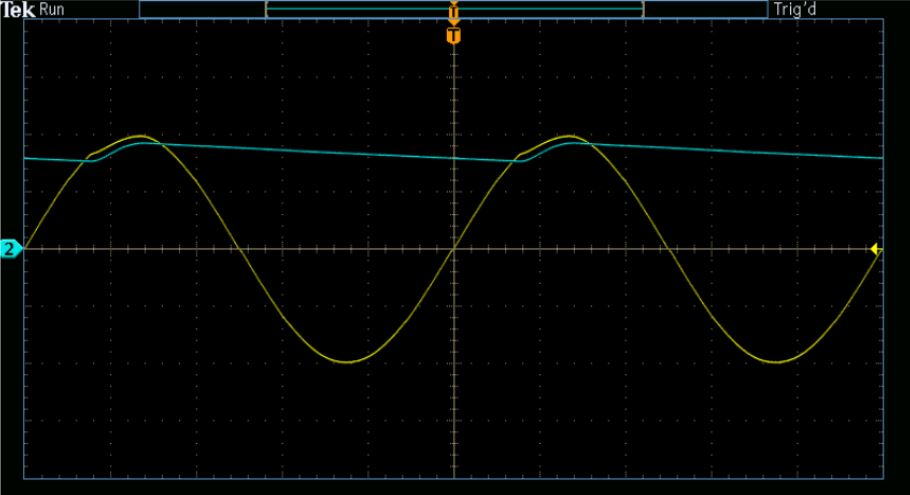
\includegraphics[scale=0.6]{../assets/images/EL1P2/aufgabe 3 470n.JPG}
    \caption{Spannungsverlauf bei $C_L$ = 470nF}
  \end{center}
\end{figure}

\newpage

\subsection{Messung von Gesamteffektivwert, Wechseleffektivwert und des Mittelwertes von $U_1$ und $U_2$}

\begin{table}[h]
  \begin{center}
\begin{tabular}{|c|c|c|}
  \hline
  & $U_{1}$ & $U_{2}$  \\
  \hline
  U\raisebox{-0.9ex}{\~{}} & 7,053V & 2,42V\\
  \hline
  $U_{TRMS}$ & 7,053V&5,681V\\
  \hline
  $U_{DC}$ & -0.5V&5,151V\\
  \hline
\end{tabular}
\caption{Messwerte bei $C_L$ = 47nF}
\end{center}
\end{table}

\begin{table}[h]
  \begin{center}
\begin{tabular}{|c|c|c|}
  \hline
  & $U_{1}$ & $U_{2}$  \\
  \hline
  U\raisebox{-0.9ex}{\~{}} & 7,053V & 1,756V\\
  \hline
  $U_{TRMS}$ & 7,053V & 6,63V\\
  \hline
  $U_{DC}$ & -0.5V  & 6,414\\
  \hline
\end{tabular}
\caption{Messwerte bei $C_L$ = 470nF}
\end{center}
\end{table}

\subsection{Welligkeit von $U_2$}

Die Welligkeit ist definiert als das Verhältnis vom Effektivwert des Wechselanteils U\raisebox{-0.9ex}{\~{}} zum Betrag des Gleichanteils $U_{DC}$:

\begin{align*}
  r_u = \frac{U\raisebox{-0.9ex}{\~{}}}{|U_{DC}|}
\end{align*}

Für $C_L$ = 47nF gilt ergibt sich folgende Welligkeit der Spannung:
\begin{align*}
  r_u = \frac{2,42V}{5,151V} = 0,47
\end{align*}
Und für $C_L$ = 470nF:
\begin{align*}
  r_u = \frac{1,756V}{6,414V} = 0,27
\end{align*}

Je kleiner die Welligkeit, desto stärker die Glättung des Signals. Diese Glättung ist abhängig von der Kapazität des Kondensators, je größer sie ist, desto besser die Glättung und kleiner die Welligkeit.
\\ In der Nachbereitung ist aufgefallen, dass die gemessenen Spannungen bei $U_2$ für $C_L$ = 470nF zu gering sind. Dies kann an der Auswahl eines falschen Kondensators liegen.
Dennoch lässt sich trotzdem erkennen, dass die Werte größer sind als bei der kleineren Kapazität.

\section{Zweiweggleichrichterschaltung}

\begin{task}
  TIn dem letzten Versuch wollen wir nun die Eigenschaften einer Zweiweggleichrichterschaltung mithilfe der uns vermittelten
  Methoden analysieren und auswerten.
\end{task}

\begin{devlist}
  T\begin{itemize}
    \item Oszilloskop
    \item Funktionsgenerator
    \item Multimeter
    \item Lastwiderstand
    \item Kondensator
    \item 1N4148 Siliziumdiode
  \end{itemize}
\end{devlist}

\begin{figure}[h]
  \begin{center}
    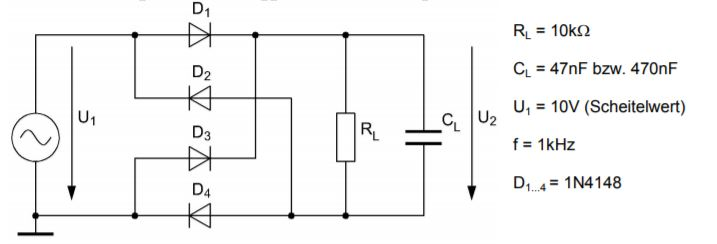
\includegraphics{../assets/images/EL1P2/aufgabe 4 schaltung.JPG}
    \caption{Zweiweggleichrichterschaltung}
  \end{center}
\end{figure}

\newpage

\subsection{Darstellung der Zeitverläufe von $U_1$ und $U_2$}

\begin{figure}[h]
  \begin{center}
    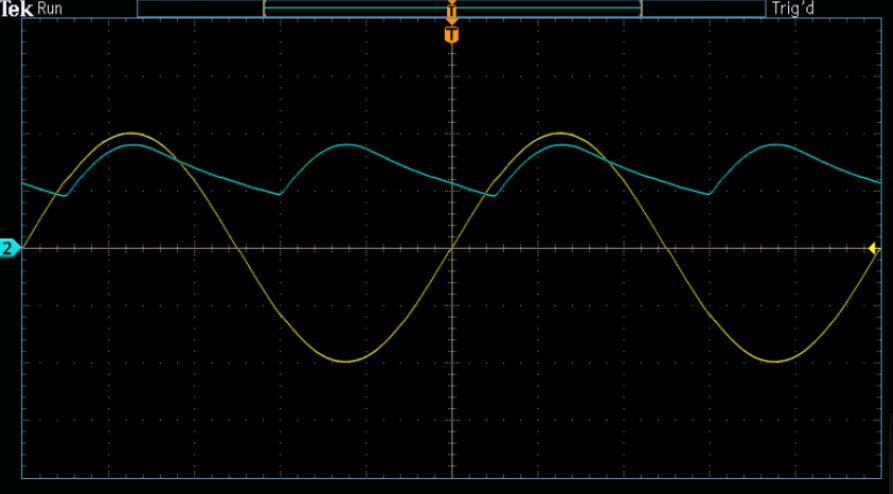
\includegraphics[scale=0.7]{../assets/images/EL1P2/aufgabe 4 47n.JPG}
    \caption{Spannungsverlauf bei $C_L$ = 47nF}
  \end{center}
\end{figure}

\begin{figure}[h]
  \begin{center}
    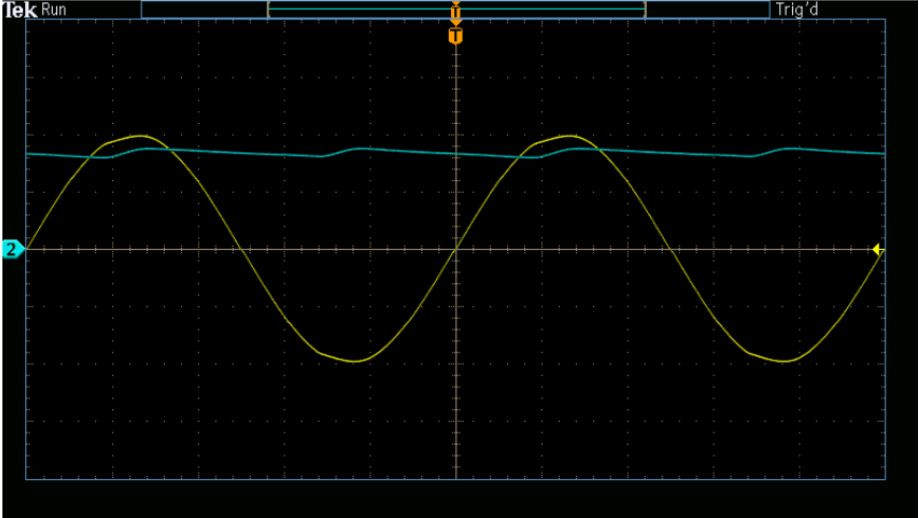
\includegraphics[scale=0.6]{../assets/images/EL1P2/aufgabe 4 470n.JPG}
    \caption{Spannungsverlauf bei $C_L$ = 470nF}
  \end{center}
\end{figure} 

\newpage

\subsection{Messung von Gesamteffektivwert, Wechseleffektivwert und des Mittelwertes von $U_1$ und $U_2$}

\begin{table}[h]
  \begin{center}
\begin{tabular}{|c|c|c|}
  \hline
  & $U_{1}$ & $U_{2}$  \\
  \hline
  U\raisebox{-0.9ex}{\~{}} & 7,012V & 1,441V\\
  \hline
  $U_{TRMS}$ & 7,012V&7,42V\\
  \hline
  $U_{DC}$ & -0.53V&7,382V\\
  \hline
\end{tabular}
\caption{Messwerte bei $C_L$ = 47nF}
\end{center}
\end{table}

\begin{table}[h]
  \begin{center}
\begin{tabular}{|c|c|c|}
  \hline
  & $U_{1}$ & $U_{2}$  \\
  \hline
  U\raisebox{-0.9ex}{\~{}} & 7,012V & 0,21V\\
  \hline
  $U_{TRMS}$ & 7,012V & 8,172V\\
  \hline
  $U_{DC}$ & -0.53V  & 8,172V\\
  \hline
\end{tabular}
\caption{Messwerte bei $C_L$ = 470nF}
\end{center}
\end{table}

\subsection{Welligkeit von $U_2$}

Ganz analog zu Versuch 3 wird nun wieder die Welligkeit bestimmt:

\begin{align*}
  r_u = \frac{U\raisebox{-0.9ex}{\~{}}}{|U_{DC}|}
\end{align*}

Für $C_L$ = 47nF gilt ergibt sich folgende Welligkeit der Spannung:
\begin{align*}
  r_u = \frac{1,441V}{7,382} = 0,2
\end{align*}
Und für $C_L$ = 470nF:
\begin{align*}
  r_u = \frac{0,21}{8,172} = 0,026
\end{align*}

Im Vergleich zur Einweggleichrichterschaltung ergibt sich eine noch geringere Welligkeit und damit ein noch besseres gleichgerichtetes Signal.
Durch die Verschaltung von vier Dioden kommt es zu keinem Zeitpunkt zu einer kompletten Sperrung der Quellspannung $U_1$.

\end{document}
